\documentclass[aspectratio=169, 10pt]{beamer}

% --- Theme & Color Configuration ---
\usetheme{Madrid}
\usefonttheme{professionalfonts}
\setbeamertemplate{navigation symbols}{}
\setbeamertemplate{headline}{}

% Custom Color Palette
\definecolor{darkslate}{RGB}{30, 41, 59}
\definecolor{lightbg}{RGB}{248, 250, 252}
\definecolor{mathred}{RGB}{192, 41, 43}
\definecolor{accentblue}{RGB}{30, 110, 180}
\definecolor{darkgreen}{RGB}{34, 139, 34}
\definecolor{ulbblue}{RGB}{0, 51, 102}
\definecolor{amber}{RGB}{217, 119, 6}

\setbeamercolor{structure}{fg=ulbblue}
\setbeamercolor{palette primary}{bg=ulbblue, fg=white}
\setbeamercolor{palette secondary}{bg=accentblue, fg=white}
\setbeamercolor{palette tertiary}{bg=darkslate, fg=white}
\setbeamercolor{palette quaternary}{bg=ulbblue, fg=white}
\setbeamercolor{titlelike}{parent=palette primary, fg=white}
\setbeamercolor{frametitle}{bg=ulbblue, fg=white}
\setbeamercolor{block title}{bg=ulbblue!15, fg=ulbblue}
\setbeamercolor{block body}{bg=lightbg, fg=darkslate}
\setbeamercolor{block title alerted}{bg=mathred!15, fg=mathred}
\setbeamercolor{block body alerted}{bg=lightbg, fg=darkslate}
\setbeamercolor{block title example}{bg=darkgreen!15, fg=darkgreen}
\setbeamercolor{block body example}{bg=lightbg, fg=darkslate}

% --- Packages ---
\usepackage[utf8]{inputenc}
\usepackage[T1]{fontenc}
\usepackage{amsmath, amssymb, amsfonts, mathtools}
\usepackage{bm}
\usepackage{booktabs}
\usepackage{tikz}
\usepackage{pgfplots}
\pgfplotsset{compat=1.18}
\usetikzlibrary{arrows.meta, positioning, calc, patterns}

\usepackage{mathtools}  
\mathtoolsset{showonlyrefs} % TO REMOVE QUEATION NUMBERING IF NOT CITED/REFERENCED

\title[Quasi-Static Limits at 26\,GHz]{Quasi-Static Limits \& Doppler Spectrum at 26\,GHz}
\subtitle{ELEC-H415 (Chapter 4)}
\author[Lucas Placentino]{Lucas Placentino}
\institute[ULB]{École Polytechnique de Bruxelles \\ Université libre de Bruxelles}
\date{2026}

\begin{document}

% ==============================================================================
% SLIDE 1: Title Slide
% ==============================================================================
\begin{frame}
    \titlepage
    % \begin{center}
    %     \footnotesize \textbf{Focus:} Microscopic Doppler Shift, Coherence Metrics ($\Delta t_c, \Delta d_c$), and Quasi-Static Breakdown
    % \end{center}
\end{frame}

% ==============================================================================
% SLIDE 2: Problem Statement & Quasi-Static Approximation
% ==============================================================================
\begin{frame}{Physical Context: The Quasi-Static Hypothesis at 26\,GHz}
\small
    \begin{columns}[T]
        \begin{column}{0.56\textwidth}
            \begin{block}{\small The Quasi-Static Approximation (Course Definition)}
                In telecommunication systems, the channel is assumed \textbf{time-invariant} during the transmission of a block of symbols of duration $t_s$:
                \begin{equation}
                    y(t) = h(t) x(t) \quad \xrightarrow{t_s \ll \Delta t_c} \quad y(t) \simeq h \cdot x(t)
                \end{equation}
                We speak about a \textbf{slow fading channel}.
            \end{block}
            \begin{alertblock}{\small The mmWave Physical Challenge}
                At carrier frequency $f_c = 26\text{ GHz}$:
                \begin{equation}
                    \lambda = \frac{c}{f_c} = \frac{3 \times 10^8\text{ m/s}}{26 \times 10^9\text{ Hz}} \approx \mathbf{1.154\text{ cm}}
                \end{equation}
                Because $\lambda$ is on the centimeter scale, does the quasi-static assumption remain valid for a moving receiver?
            \end{alertblock}
        \end{column}

        \begin{column}{0.42\textwidth}
            \begin{center}
            \begin{figure}
                \centering
                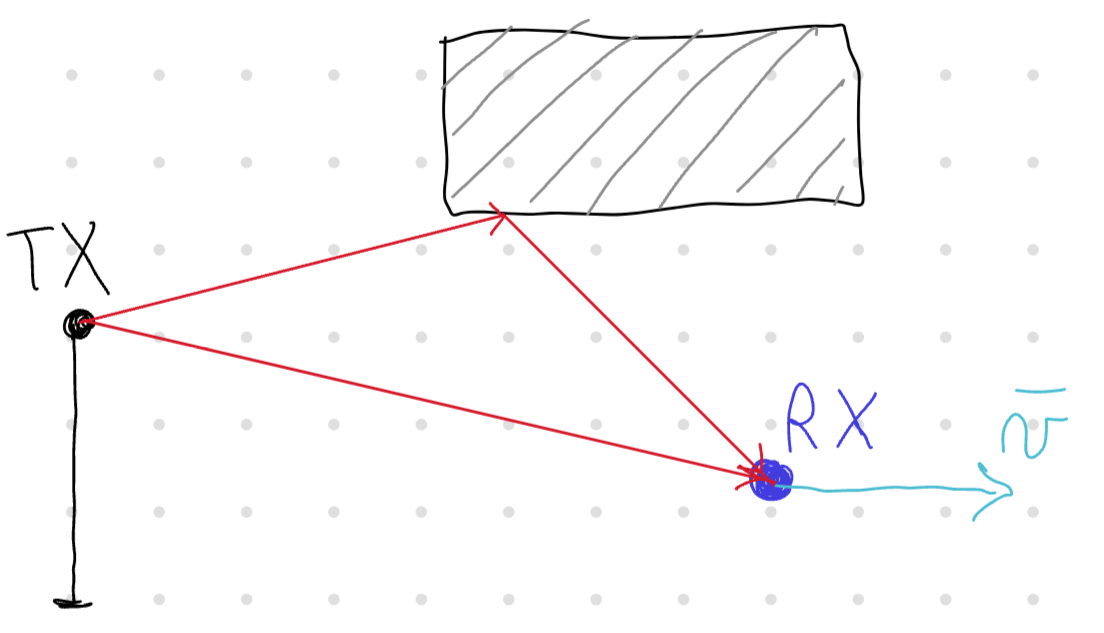
\includegraphics[width=0.85\linewidth]{chap4-fig.png}
            \end{figure}
            Wavelength $\lambda = 1.15\text{ cm}$\\$\implies$ Millimeter-scale phase shifts
            % \begin{tikzpicture}[scale=0.75, every node/.style={transform shape}]
            %     % Transmitter
            %     \draw[thick, fill=gray!20] (-0.5,0) rectangle (0.5,0.8);
            %     \draw[ultra thick, ulbblue] (0,0.8) -- (0,2.4);
            %     \node at (0,2.7) {\textbf{TX (26 GHz)}};
            %     \draw[thick, red] (0,2.4) -- (-0.2,2.7);
            %     \draw[thick, red] (0,2.4) -- (0.2,2.7);
                
            %     % Obstacle / IO
            %     \draw[thick, fill=darkslate!15] (1.8,1.2) rectangle (3.2,3.5);
            %     \node at (2.5,2.35) {\textbf{IO}};
                
            %     % Receiver
            %     \draw[thick, fill=amber!20] (3.8,-0.2) rectangle (4.6,0.5);
            %     \node at (4.2,0.15) {\textbf{RX}};
            %     \draw[-{Stealth[length=2.5mm]}, very thick, mathred] (4.6,0.15) -- (5.7,0.15) node[midway, above] {$\vec{v}$};
                
            %     % Multipath Rays
            %     \draw[thick, darkgreen, -{Stealth[length=2mm]}] (0,2.4) -- (3.8,0.4) node[midway, below, sloped] {\scriptsize Direct ray};
            %     \draw[thick, accentblue, dashed] (0,2.4) -- (1.8,2.8);
            %     \draw[thick, accentblue, -{Stealth[length=2mm]}] (1.8,2.8) -- (3.9,0.5) node[midway, above, sloped] {\scriptsize Reflected ray};
                
            %     \node[font=\scriptsize, align=center, red] at (2.5,-0.8) {Wavelength $\lambda = 1.15\text{ cm}$\\$\implies$ Millimeter-scale phase shifts};
            % \end{tikzpicture}
            \end{center}
        \end{column}
    \end{columns}
\end{frame}

% ==============================================================================
% SLIDE 3: Moving in a Local Area: Plane Wave Phase Geometry
% ==============================================================================
\begin{frame}{Local Area Formulation}
\small
    \begin{columns}[T]
        \begin{column}{0.54\textwidth}
        \vspace{-1.2em}
            \begin{definition}[Local Area]
                A region of space where the received signal is made of a given set of $N$ plane waves of \textbf{constant amplitudes} $a_n$.
            \end{definition}
            
            Let the receiver move along trajectory $\vec{r}(t)$.
            At the origin ($\vec{r} = \vec{0}$), each Multipath Component (MPC) $n$ has delay $\tau_{n0}$ and phase $\phi_{n0}$.
            When moving, its phase changes as a plane wave:
            \begin{equation}
                e^{j\phi_n(t)} e^{-j2\pi f_c \tau_n} = \underbrace{e^{j\phi_{n0}} e^{-j2\pi f_c \tau_{n0}}}_{\triangleq \, e^{j\varphi_n}} e^{-j\vec{\beta}_n \cdot \vec{r}(t)}
            \end{equation}
            where $\varphi_n = \phi_{n0} - 2\pi f_c \tau_{n0}$.

            \begin{block}{Local Area Channel Transfer Function}
                \begin{equation}
                    \boxed{h(t) = \sum_{n=1}^{N} a_n e^{j\varphi_n} e^{-j\vec{\beta}_n \cdot \vec{r}(t)}}
                \end{equation}
            \end{block}
        \end{column}

        \begin{column}{0.44\textwidth}
            \begin{center}
            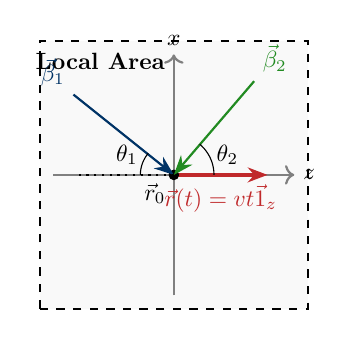
\begin{tikzpicture}[scale=0.85, every node/.style={transform shape}]
                % Local Area Box
                \draw[thick, dashed, fill=gray!5] (-2,-2) rectangle (2,2);
                \node at (-1.1,1.7) {\textbf{Local Area}};
                
                % Coordinates
                \draw[->, thick, gray] (-1.8,0) -- (1.8,0) node[right, black] {$z$};
                \draw[->, thick, gray] (0,-1.8) -- (0,1.8) node[above, black] {$x$};
                
                % Trajectory along z
                \draw[ultra thick, mathred, -{Stealth[length=2.5mm]}] (0,0) -- (1.4,0) node[midway, below] {$\vec{r}(t) = v t \vec{1}_z$};
                \filldraw[black] (0,0) circle (2pt) node[below left] {$\vec{r}_0$};
                
                % Plane Wave 1
                \draw[thick, ulbblue, {Stealth[length=2.5mm]}-] (0,0) -- (-1.5,1.2) node[above left] {$\vec{\beta}_1$};
                \draw[thick, dotted] (0,0) -- (-1.5,0);
                \draw[domain=140:180] plot ({0.5*cos(\x)}, {0.5*sin(\x)});
                \node at (-0.7,0.3) {$\theta_1$};

                % Plane Wave 2
                \draw[thick, darkgreen, {Stealth[length=2.5mm]}-] (0,0) -- (1.2,1.4) node[above right] {$\vec{\beta}_2$};
                \draw[domain=0:50] plot ({0.6*cos(\x)}, {0.6*sin(\x)});
                \node at (0.8,0.3) {$\theta_2$};
            \end{tikzpicture}
            \end{center}
        \end{column}
    \end{columns}
\end{frame}

% ==============================================================================
% SLIDE 4: Single MPC Doppler Shift Derivation
% ==============================================================================
\begin{frame}{Step-by-Step Derivation of the Doppler Shift}
    Let the receiver move at constant speed $v$ along the $z$-axis: $\vec{r}(t) = v t \vec{1}_z$.
    Consider a single plane wave ($N=1$) with amplitude $a=1$ arriving at angle $\theta$ relative to the $z$-axis:

    \begin{columns}[T]
        \begin{column}{0.5\textwidth}
            \textbf{1. Wavevector Definition:}
            \begin{equation}
                \vec{\beta} = -\beta \cos\theta \, \vec{1}_z - \beta \sin\theta \, \vec{1}_x
            \end{equation}
            where $\beta = \frac{\omega_c}{c} = \frac{2\pi}{\lambda}$ is the wavenumber.

            \textbf{2. Spatial Inner Product:}
            \begin{equation}
                \vec{\beta} \cdot \vec{r}(t) = \left( -\beta \cos\theta \, \vec{1}_z \right) \cdot \left( v t \, \vec{1}_z \right) = -\beta v t \cos\theta
            \end{equation}

            \textbf{3. Channel Transfer Function:}
            \begin{equation}
                h(t) = e^{-j\vec{\beta} \cdot \vec{r}(t)} = e^{j\beta v \cos\theta \cdot t} = e^{j\omega_D t}
            \end{equation}
        \end{column}
\vspace{-1em}
        \begin{column}{0.48\textwidth}
            \begin{block}{Doppler Angular Frequency ($\omega_D$)}
                \begin{equation}
                    \boxed{\omega_D \triangleq \beta v \cos\theta = \frac{2\pi}{\lambda} v \cos\theta}
                \end{equation}
            \end{block}
\vspace{-1em}
            \begin{alertblock}{Maximal Doppler Shift ($f_m$)}
                Obtained for head-on incidence ($\theta = 0 \implies \cos\theta = 1$):
                \begin{equation}
                    \boxed{f_m \triangleq \frac{\omega_m}{2\pi} = \frac{\beta v}{2\pi} = \frac{v}{\lambda} = \frac{v f_c}{c}}
                \end{equation}
            \end{alertblock}
            The Doppler frequency shift is bounded by:
            \vspace{-1em}
            \begin{equation*}
                f_D \in [-f_m, \, +f_m]
            \end{equation*}
        \end{column}
    \end{columns}
\end{frame}

% ==============================================================================
% SLIDE 5: Continuous Wave (CW) Transmission
% ==============================================================================
\begin{frame}{Physical Interpretation: Continuous Wave (CW) Transmission}
\small
    Consider an unmodulated unit-amplitude carrier transmission: $x(t) = 1$.
    
    \begin{columns}[T]
        \begin{column}{0.52\textwidth}
            \textbf{Baseband Output:}
            \begin{equation}
                y(t) = h(t) x(t) = h(t) = e^{j\omega_D t}
            \end{equation}
            \textbf{Physical Real RF Received Signal:}
            \begin{align}
                y_{\text{RF}}(t) &= \text{Re}\left\{ y(t) e^{j\omega_c t} \right\} = \text{Re}\left\{ e^{j\omega_D t} e^{j\omega_c t} \right\} \nonumber \\
                                 &= \text{Re}\left\{ e^{j(\omega_c + \omega_D)t} \right\} \nonumber \\
                                 &= \boxed{\cos\Big( (\omega_c + \omega_D) t \Big)}
            \end{align}
            \begin{block}{Physical Interpretation}
                The carrier frequency is shifted from $f_c$ to $f_c + f_D$. The channel acts as a frequency modulator through receiver velocity.
            \end{block}
        \end{column}

        \begin{column}{0.46\textwidth}
            \begin{center}
            \begin{tikzpicture}[scale=0.72, every node/.style={transform shape}]
                % TX Spectrum
                \begin{axis}[
                    width=6.0cm, height=3.2cm,
                    axis lines=middle, xlabel={$f$}, ylabel={$|X_{\text{RF}}(f)|$},
                    xmin=24, xmax=28, ymin=0, ymax=1.3,
                    ticks=none, xlabel style={right}, ylabel style={above}
                ]
                    \draw[ultra thick, ulbblue, -{Stealth[length=2mm]}] (axis cs: 26,0) -- (axis cs: 26,1.0);
                    \node[below, font=\scriptsize] at (axis cs: 26,0) {$f_c = 26\text{ GHz}$};
                \end{axis}
            \end{tikzpicture}
            
            \vspace{0.1cm}
            \begin{tikzpicture}[scale=0.72, every node/.style={transform shape}]
                % RX Spectrum
                \begin{axis}[
                    width=6.0cm, height=3.2cm,
                    axis lines=middle, xlabel={$f$}, ylabel={$|Y_{\text{RF}}(f)|$},
                    xmin=24, xmax=28, ymin=0, ymax=1.3,
                    ticks=none, xlabel style={right}, ylabel style={above}
                ]
                    \draw[ultra thick, mathred, -{Stealth[length=2mm]}] (axis cs: 26.6,0) -- (axis cs: 26.6,1.0);
                    \draw[dashed, gray] (axis cs: 26,0) -- (axis cs: 26,1.0);
                    \node[below, font=\scriptsize, gray] at (axis cs: 26,0) {$f_c$};
                    \node[below, font=\scriptsize, mathred] at (axis cs: 26.6,0) {$f_c + f_D$};
                    \draw[{Stealth[length=1.5mm]}-{Stealth[length=1.5mm]}, thick, darkslate] (axis cs: 26,0.5) -- (axis cs: 26.6,0.5) node[midway, above, font=\tiny] {$f_D$};
                \end{axis}
            \end{tikzpicture}
            \end{center}
        \end{column}
    \end{columns}
\end{frame}

% ==============================================================================
% SLIDE 6: The Multipath Doppler Spectrum
% ==============================================================================
\begin{frame}{The Doppler Spectrum for $N$ Multipath Components}
\small
    When $N$ multipaths arrive simultaneously from angles $\theta_n$:
    \begin{equation}
        h(t) = \sum_{n=1}^{N} a_n e^{j\varphi_n} e^{j\omega_{Dn} t} \quad \text{with} \quad \omega_{Dn} = \beta v \cos\theta_n = 2\pi f_m \cos\theta_n
    \end{equation}

    \begin{columns}[T]
        \begin{column}{0.5\textwidth}
            \begin{block}{Spectral Representation of $h(t)$}
                \begin{equation}
                    H(f) = \mathcal{F}\{h(t)\} = \sum_{n=1}^{N} a_n e^{j\varphi_n} \delta(f - f_{Dn})
                \end{equation}
                The received spectrum is spread over a finite bandwidth called the \textbf{Doppler Spread}:
                \begin{equation}
                    \boxed{B_D = 2 f_m = \frac{2v}{\lambda} = \frac{2 v f_c}{c}}
                \end{equation}
            \end{block}
            This Doppler spectrum characterizes the \textbf{rate of time variation} of the channel alone.
        \end{column}

        \begin{column}{0.48\textwidth}
            \begin{center}
            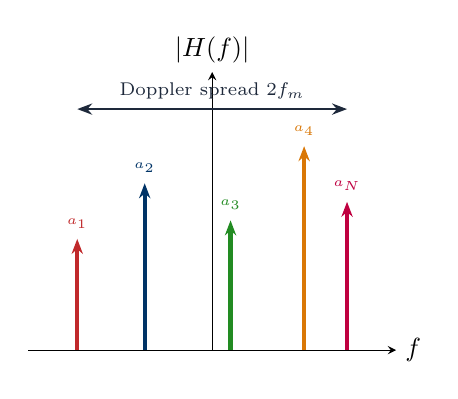
\begin{tikzpicture}[scale=0.95, every node/.style={transform shape}]
                \begin{axis}[
                    width=6.5cm, height=5.3cm,
                    axis lines=middle,
                    xlabel={$f$}, ylabel={$|H(f)|$},
                    xmin=-3, xmax=3, ymin=0, ymax=1.5,
                    ticks=none,
                    xlabel style={right}, ylabel style={above}
                ]
                    % Peaks
                    \draw[ultra thick, mathred, -{Stealth[length=2mm]}] (axis cs: -2.2,0) -- (axis cs: -2.2,0.6) node[above, font=\tiny] {$a_1$};
                    \draw[ultra thick, ulbblue, -{Stealth[length=2mm]}] (axis cs: -1.1,0) -- (axis cs: -1.1,0.9) node[above, font=\tiny] {$a_2$};
                    \draw[ultra thick, darkgreen, -{Stealth[length=2mm]}] (axis cs: 0.3,0) -- (axis cs: 0.3,0.7) node[above, font=\tiny] {$a_3$};
                    \draw[ultra thick, amber, -{Stealth[length=2mm]}] (axis cs: 1.5,0) -- (axis cs: 1.5,1.1) node[above, font=\tiny] {$a_4$};
                    \draw[ultra thick, purple, -{Stealth[length=2mm]}] (axis cs: 2.2,0) -- (axis cs: 2.2,0.8) node[above, font=\tiny] {$a_N$};
                    
                    % Labels
                    \node[below, font=\scriptsize] at (axis cs: 0,0) {$0$};
                    \node[below, font=\scriptsize, mathred] at (axis cs: -2.2,0) {$-f_m$};
                    \node[below, font=\scriptsize, purple] at (axis cs: 2.2,0) {$+f_m$};
                    
                    % Arrow
                    \draw[{Stealth[length=2mm]}-{Stealth[length=2mm]}, thick, darkslate] (axis cs: -2.2,1.3) -- (axis cs: 2.2,1.3) node[midway, above, font=\scriptsize] {Doppler spread $2f_m$};
                \end{axis}
            \end{tikzpicture}
            \end{center}
        \end{column}
    \end{columns}
\end{frame}

% ==============================================================================
% SLIDE 7: Channel Coherence Time
% ==============================================================================
\begin{frame}{Channel Coherence Time ($\Delta t_c$)}
    \begin{columns}[T]
        \begin{column}{0.54\textwidth}
        \vspace{-1em}
            \begin{block}{Derivation from Spectral Spread}
                \small
                As with any function of time, the time-scale of variation of $h(t)$ is inversely proportional to its spectral width ($2f_m$):
                \begin{equation}
                    \boxed{\Delta t_c \simeq \frac{1}{2 f_m} = \frac{1}{2}\frac{\lambda}{v}}
                \end{equation}
            \end{block}

            \begin{alertblock}{Condition for Quasi-Static Fading}
            \small
                Let $t_s$ be the duration of a transmitted block of symbols:
                \begin{itemize}
                    \item If $\mathbf{t_s \ll \Delta t_c}$: The channel is constant over the block $\implies$ \textbf{Slow Fading} (quasi-static approximation holds).
                    \item If $\mathbf{t_s \sim \Delta t_c}$ or $\mathbf{t_s > \Delta t_c}$: The channel varies during transmission $\implies$ \textbf{Fast Fading} (quasi-static approximation fails).
                \end{itemize}
            \end{alertblock}
        \end{column}

        \begin{column}{0.44\textwidth}
            \begin{center}
            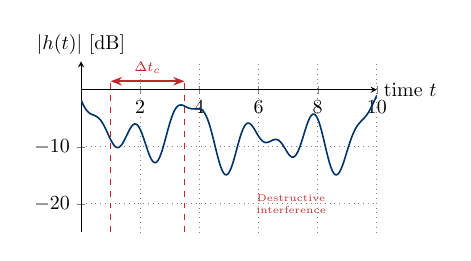
\begin{tikzpicture}[scale=0.72, every node/.style={transform shape}]
                \begin{axis}[
                    width=6.8cm, height=4.6cm,
                    axis lines=middle,
                    xlabel={time $t$}, ylabel={$|h(t)|$ [dB]},
                    xmin=0, xmax=10, ymin=-25, ymax=5,
                    grid=both, grid style={dotted, gray},
                    xlabel style={right}, ylabel style={above}
                ]
                    \addplot[domain=0:10, samples=200, thick, ulbblue] 
                        { -5 + 4*cos(deg(1.8*x)) + 3*cos(deg(3.1*x + 1)) + 2*sin(deg(5.2*x - 2)) - 3/(1 + 0.5*(x-3.2)^2) - 8/(1 + 2*(x-7.1)^2) };
                    
                    % Coherence interval
                    \draw[{Stealth[length=2mm]}-{Stealth[length=2mm]}, thick, mathred] (axis cs: 1.0, 1.5) -- (axis cs: 3.5, 1.5) node[midway, above, font=\scriptsize] {$\Delta t_c$};
                    \draw[dashed, mathred] (axis cs: 1.0, -25) -- (axis cs: 1.0, 1.5);
                    \draw[dashed, mathred] (axis cs: 3.5, -25) -- (axis cs: 3.5, 1.5);
                    
                    \node[font=\tiny, mathred, align=center] at (axis cs: 7.1, -20) {Destructive\\interference};
                \end{axis}
            \end{tikzpicture}
            \end{center}
            \vspace{-0.2cm}
            \footnotesize Interference pattern causes fast fading in time as the receiver moves.
        \end{column}
    \end{columns}
\end{frame}

% ==============================================================================
% SLIDE 8: Spatial Coherence Distance & Standing Waves
% ==============================================================================
\begin{frame}{Spatial Coherence Distance ($\Delta d_c$) \& Standing Waves}
\small
    \begin{columns}[T]
        \begin{column}{0.54\textwidth}
            \textbf{Coherence Distance Definition:}
            The spatial distance traveled by the receiver at speed $v$ during the coherence time $\Delta t_c$: 
           \vspace{-1em}
           \begin{equation}
                \boxed{\Delta d_c = v \cdot \Delta t_c = v \left(\frac{1}{2}\frac{\lambda}{v}\right) = \frac{\lambda}{2}}
            \end{equation}
\vspace{-1em}
            \begin{block}{Proof via 2-Ray Standing Wave}
            \small
                Two equal-amplitude waves arriving in opposite directions along $z$ ($\theta_1 = 0$, $\theta_2 = \pi$):
                \begin{equation}
                    h(z) = e^{-j\beta z} + e^{+j\beta z} = 2\cos(\beta z)
                \end{equation}
                The power pattern is:
                \begin{equation}
                    |h(z)|^2 = 4\cos^2\left(\frac{2\pi}{\lambda} z\right) = 2\left[1 + \cos\left(\frac{4\pi}{\lambda} z\right)\right]
                \end{equation}
                The spatial power period is $\frac{\lambda}{2}$. Peak to destructive null is $\frac{\lambda}{4}$.
            \end{block}
        \end{column}

        \begin{column}{0.44\textwidth}
            \begin{center}
            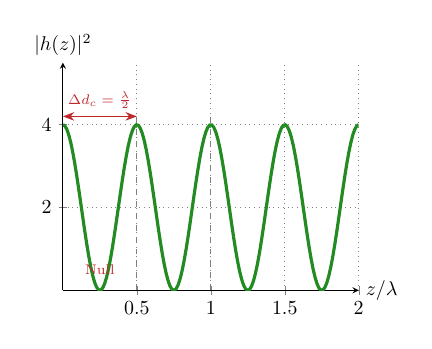
\begin{tikzpicture}[scale=0.72, every node/.style={transform shape}]
                \begin{axis}[
                    width=6.8cm, height=5.6cm,
                    axis lines=middle,
                    xlabel={$z / \lambda$}, ylabel={$|h(z)|^2$},
                    xmin=0, xmax=2.0, ymin=0, ymax=5.5,
                    grid=both, grid style={dotted, gray},
                    xlabel style={right}, ylabel style={above}
                ]
                    \addplot[domain=0:2.0, samples=150, ultra thick, darkgreen] { 4*(cos(deg(2*pi*x)))^2 };
                    
                    % Lambda/2 marker
                    \draw[{Stealth[length=2mm]}-{Stealth[length=2mm]}, thick, mathred] (axis cs: 0, 4.2) -- (axis cs: 0.5, 4.2) node[midway, above, font=\scriptsize] {$\Delta d_c = \frac{\lambda}{2}$};
                    \draw[dashed, gray] (axis cs: 0.5, 0) -- (axis cs: 0.5, 4.2);
                    \draw[dashed, gray] (axis cs: 1.0, 0) -- (axis cs: 1.0, 4.2);
                    
                    \node[font=\scriptsize, mathred] at (axis cs: 0.25, 0.5) {Null};
                \end{axis}
            \end{tikzpicture}
            \end{center}
            \vspace{-0.2cm}
            \footnotesize \textbf{Spatial scale at 26 GHz:}
            $$\Delta d_c = \frac{11.54\text{ mm}}{2} = \mathbf{5.77\text{ mm}}$$
        \end{column}
    \end{columns}
\end{frame}

% ==============================================================================
% SLIDE 9: Quantitative Computation at 26 GHz
% ==============================================================================
\begin{frame}{Applied Calculations: 26\,GHz mmWave Mobility Limits}
    \begin{block}{System Parameters}
        Carrier frequency: $f_c = 26\text{ GHz} \implies \lambda = \frac{3\times 10^8}{26\times 10^9} = 0.01154\text{ m} = \mathbf{11.54\text{ mm}}$.
    \end{block}

    \begin{table}
        \centering
        \small
        \footnotesize
        \begin{tabular}{@{}lcccccl@{}}
            \toprule
            \textbf{Scenario} & $\bm{v}$ \textbf{[km/h]} & $\bm{v}$ \textbf{[m/s]} & $\bm{f_m = \frac{v}{\lambda}}$ & $\bm{\Delta t_c = \frac{1}{2f_m}}$ & $\bm{\Delta d_c}$ & \textbf{Quasi-Static Status ($t_s = 0.125\text{ ms}$)} \\
            \midrule
            \textbf{Pedestrian}       & 5   & 1.39  & $120.4\text{ Hz}$  & $\mathbf{4.15\text{ ms}}$   & $5.77\text{ mm}$ & \textcolor{darkgreen}{\textbf{Valid: $t_s \ll \Delta t_c$}} ($t_s \approx 3\% \Delta t_c$) \\
            \textbf{City Vehicle}     & 50  & 13.89 & $1.204\text{ kHz}$ & $\mathbf{415.4\ \mu\text{s}}$ & $5.77\text{ mm}$ & \textcolor{amber}{\textbf{Marginal: $t_s < \Delta t_c$}} ($t_s \approx 30\% \Delta t_c$) \\
            \textbf{Highway}    & 120 & 33.33 & $2.889\text{ kHz}$ & $\mathbf{173.1\ \mu\text{s}}$ & $5.77\text{ mm}$ & \textcolor{mathred}{\textbf{Critical: $t_s \sim \Delta t_c$}} ($t_s \approx 72\% \Delta t_c$) \\
            \textbf{TGV} & 300 & 83.33 & $7.222\text{ kHz}$ & $\mathbf{69.2\ \mu\text{s}}$  & $5.77\text{ mm}$ & \textcolor{mathred}{\textbf{Breakdown: $t_s > \Delta t_c$}} ($t_s \approx 181\% \Delta t_c$) \\
            \bottomrule
        \end{tabular}
    \end{table}

    \begin{alertblock}{Key Analytical Finding}
        At 26 GHz, for a typical transmission block $t_s = 0.125\text{ ms}$, the quasi-static approximation breaks down for speeds above $v \approx 166\text{ km/h}$, as $\Delta t_c$ drops below $t_s$.
    \end{alertblock}
\end{frame}

% ==============================================================================
% SLIDE 10: Parametric Coherence Curve vs. Speed
% ==============================================================================
\begin{frame}{Coherence Time vs. Velocity: Breakdown Boundaries}
    \begin{center}
    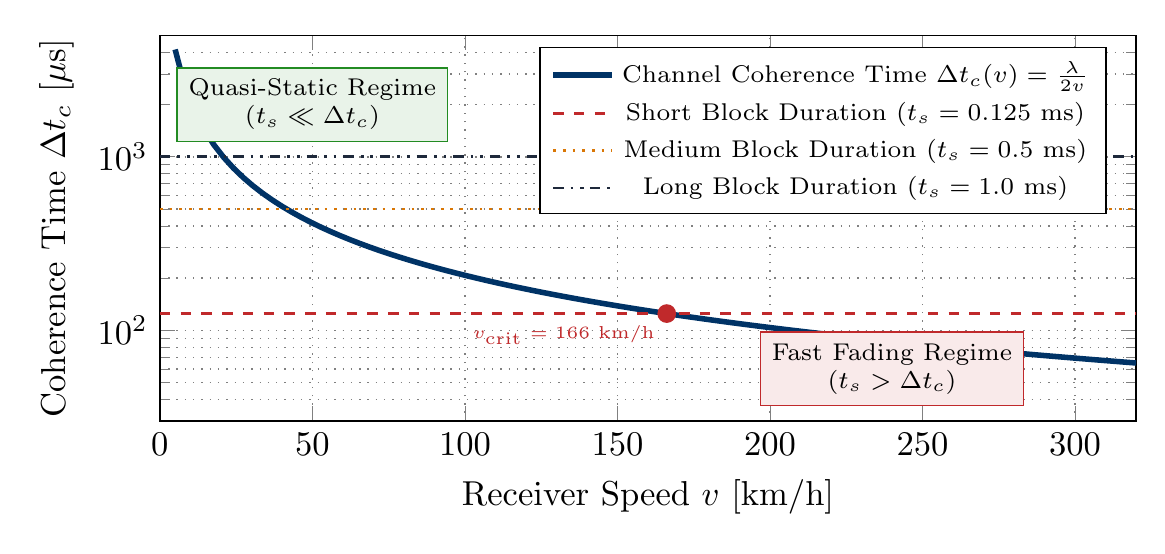
\begin{tikzpicture}[scale=1.25]
        \begin{axis}[
            width=11.5cm, height=5.5cm,
            xlabel={Receiver Speed $v$ [km/h]},
            ylabel={Coherence Time $\Delta t_c$ [$\mu$s]},
            xmin=0, xmax=320,
            ymin=30, ymax=5000,
            ymode=log,
            grid=both, grid style={dotted, gray},
            legend pos=north east,
            legend style={font=\scriptsize}
        ]
            % Coherence time curve: Delta t_c = lambda / (2 * v) = 20769 / v_kmh
            \addplot[domain=5:320, samples=100, ultra thick, ulbblue] { 20769 / x };
            \addlegendentry{Channel Coherence Time $\Delta t_c(v) = \frac{\lambda}{2v}$}
            
            % Horizontal reference block duration lines
            \addplot[domain=0:320, thick, mathred, dashed] { 125 };
            \addlegendentry{Short Block Duration ($t_s = 0.125\text{ ms}$)}
            
            \addplot[domain=0:320, thick, amber, dotted] { 500 };
            \addlegendentry{Medium Block Duration ($t_s = 0.5\text{ ms}$)}
            
            \addplot[domain=0:320, thick, darkslate, dashdotdotted] { 1000 };
            \addlegendentry{Long Block Duration ($t_s = 1.0\text{ ms}$)}
            
            % Intersection point for ts = 125 us
            \filldraw[mathred] (axis cs: 166.15, 125) circle (2.5pt);
            \node[below left, font=\tiny, mathred] at (axis cs: 166.15, 125) {$v_{\text{crit}} = 166\text{ km/h}$};
            
            \node[fill=mathred!10, draw=mathred, font=\scriptsize, align=center] at (axis cs: 240, 60) {Fast Fading Regime\\($t_s > \Delta t_c$)};
            \node[fill=darkgreen!10, draw=darkgreen, font=\scriptsize, align=center] at (axis cs: 50, 2000) {Quasi-Static Regime\\($t_s \ll \Delta t_c$)};
        \end{axis}
    \end{tikzpicture}
    \end{center}
\end{frame}

% ==============================================================================
% SLIDE 11: Statistical Amplitude Behavior Across Coherence Intervals
% ==============================================================================
% \begin{frame}{Statistical Envelope Behavior in the Local Area}
%     Over intervals larger than $\Delta t_c$, the phase draws randomize.
%     The complex gain $h = \sum a_n e^{j\Phi_n}$ follows:
    
%     \begin{columns}[T]
%         \begin{column}{0.5\textwidth}
%             \begin{block}{Rayleigh Fading (NLOS Case)}
%                 When no dominant path exists ($N \ge 6$):
%                 \begin{equation}
%                     f_{|h|}(r) = \frac{r}{\sigma^2} e^{-r^2 / 2\sigma^2} \quad \text{with } \mathbb{E}[|h|^2] = 2\sigma^2
%                 \end{equation}
%             \end{block}
            
%             \begin{block}{Rice Fading (LOS Case)}
%                 Dominant path $a_0$ with Rice factor $K = \frac{a_0^2}{2\sigma^2}$:
%                 \begin{equation}
%                     f_{|h|}(r) = \frac{r}{\sigma^2} e^{-\frac{r^2}{2\sigma^2} - K} I_0\left(\frac{r\sqrt{2K}}{\sigma}\right)
%                 \end{equation}
%             \end{block}
%         \end{column}

%         \begin{column}{0.48\textwidth}
%             \begin{center}
%             \begin{tikzpicture}[scale=0.72, every node/.style={transform shape}]
%                 \begin{axis}[
%                     width=6.6cm, height=4.6cm,
%                     axis lines=middle, xlabel={$|h|$}, ylabel={PDF},
%                     xmin=0, xmax=3.5, ymin=0, ymax=1.0,
%                     grid=both, grid style={dotted, gray},
%                     legend pos=north east, legend style={font=\tiny},
%                     xlabel style={right}, ylabel style={above}
%                 ]
%                     % Rayleigh (sigma = 1/sqrt(2) => 2*sigma^2 = 1)
%                     \addplot[domain=0:3.5, samples=100, thick, ulbblue] { 2*x*exp(-x^2) };
%                     \addlegendentry{Rayleigh ($K=0$)}
                    
%                     % Rice K = 4 (Exact precomputed coordinates to prevent engine errors)
%                     \addplot[smooth, thick, darkgreen] coordinates {
%                         (0.0, 0.0) (0.3, 0.005) (0.6, 0.03) (0.9, 0.12) 
%                         (1.2, 0.32) (1.4, 0.52) (1.6, 0.74) (1.8, 0.88) 
%                         (2.0, 0.92) (2.2, 0.82) (2.4, 0.61) (2.6, 0.39) 
%                         (2.8, 0.20) (3.0, 0.09) (3.2, 0.03) (3.5, 0.005)
%                     };
%                     \addlegendentry{Rice ($K=4$)}
%                 \end{axis}
%             \end{tikzpicture}
%             \end{center}
%             \vspace{-0.2cm}
%             \footnotesize \textbf{Takeaway:} The envelope $|h(t)|$ explores these probability distributions on time-scale $\Delta t_c$.
%         \end{column}
%     \end{columns}
% \end{frame}

% ==============================================================================
% SLIDE 12: Lesson Conclusion & Synthesis
% ==============================================================================
\begin{frame}{Synthesis: The mmWave Quasi-Static Chain}
    \begin{center}
    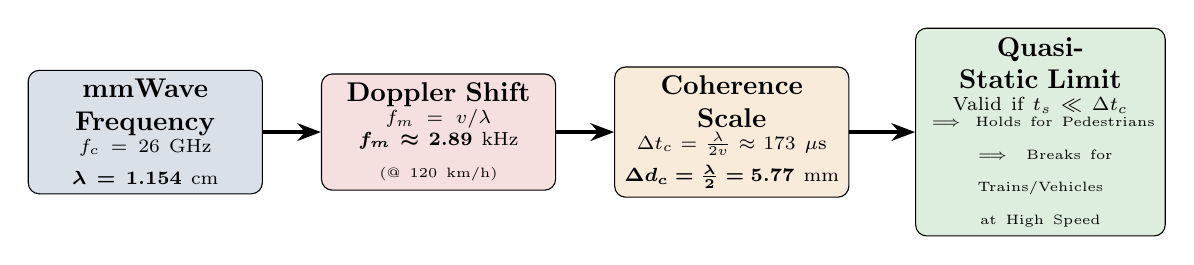
\begin{tikzpicture}[scale=0.98, every node/.style={transform shape}]
        % Nodes
        \node[draw, rectangle, fill=ulbblue!15, rounded corners, text width=2.8cm, align=center] (n1) at (0,0) {
            \textbf{mmWave Frequency}\\
            \scriptsize $f_c = 26\text{ GHz}$\\
            $\bm{\lambda = 1.154\text{ cm}}$
        };
        
        \node[draw, rectangle, fill=mathred!15, rounded corners, text width=2.8cm, align=center] (n2) at (3.8,0) {
            \textbf{Doppler Shift}\\
            \scriptsize $f_m = v/\lambda$\\
            $\bm{f_m \approx 2.89\text{ kHz}}$\\
            \tiny (@ $120\text{ km/h}$)
        };

        \node[draw, rectangle, fill=amber!15, rounded corners, text width=2.8cm, align=center] (n3) at (7.6,0) {
            \textbf{Coherence Scale}\\
            \scriptsize $\Delta t_c = \frac{\lambda}{2v} \approx 173\ \mu\text{s}$\\
            $\bm{\Delta d_c = \frac{\lambda}{2} = 5.77\text{ mm}}$
        };

        \node[draw, rectangle, fill=darkgreen!15, rounded corners, text width=3.0cm, align=center] (n4) at (11.6,0) {
            \textbf{Quasi-Static Limit}\\
            \scriptsize Valid if $t_s \ll \Delta t_c$\\
            \tiny $\implies$ Holds for Pedestrians\\
            \tiny $\implies$ Breaks for Trains/Vehicles at High Speed
        };

        % Arrows
        \draw[-{Stealth[length=3mm]}, very thick] (n1) -- (n2);
        \draw[-{Stealth[length=3mm]}, very thick] (n2) -- (n3);
        \draw[-{Stealth[length=3mm]}, very thick] (n3) -- (n4);
    \end{tikzpicture}
    \end{center}

    \vspace{0.3cm}
    \begin{block}{Key Takeaways}
        \begin{enumerate}
            \item The channel time variation is governed by the Doppler spread $2f_m = \frac{2v}{\lambda}$, defining the coherence time $\Delta t_c \simeq \frac{\lambda}{2v}$.
            \item The spatial variation period is strictly $\Delta d_c = \frac{\lambda}{2} = 5.77\text{ mm}$ at 26 GHz due to constructive and destructive interference of plane waves.
            \item The quasi-static approximation ($t_s \ll \Delta t_c$) is valid for pedestrians ($\Delta t_c = 4.15\text{ ms}$), but fails for vehicular speeds ($v > 166\text{ km/h}$ for $t_s = 125\ \mu\text{s}$), transforming the channel into a fast fading environment.
        \end{enumerate}
    \end{block}
\end{frame}

\end{document}